\glsxtrnewsymbol[description={шаг по времени, [с]}]{dt}{\ensuremath{\dt}}
\glsxtrnewsymbol[description={шаг по пространству, [м]}]{dx}{\ensuremath{\dx}}
\glsxtrnewsymbol[description={степень неявности дискретизации по времени}]{theta}{\ensuremath{\theta}}

\section{Методика численного решения}
\subsection{Аппроксимация по пространству. Метод разрывных конечных элементов}
Аппроксимацию системы 
\cref{eq:vector_system}
будем проводить методом разрывных конечных элементов~\cite{dipietro2012}.
Следуя стандартной процедуре этого метода домноженим
исходное уравнение на базисную функцию,
проинтегируем по конечному элементу $E$
применим формулу интегрирования по частям.
Получим
\begin{equation*}
\sum\limits_j M_{ij} \left(\dfr{\vec U}{t}\right)_j 
+ \sum\limits_j T_{ij} \vec F_j + \left.\vec{\bar F} \phi_i \right|_{x_l}^{x_r}
= 
\sum\limits_j M_{ij} \vec B_j.
\end{equation*}
Здесь $M_{ij}$, $T_{ij}$ -- коэффициенты матрица масс и переноса, 
\begin{equation}
\nonumber
M_{ij} = \int\phi_i\phi_j\, dx,
\qquad
T_{ij} = -\int\phi_i\dfr{\phi_j}{x}\, dx.
\end{equation}
Эти матрицы являются блочно-диагональными (или сводятся к блочнодиагональным
в результате перенумерации узлов сетки).
Значение блока этих матрицы при применении линейных и квадратичных
Лагранжевых базисных функций имеют вид:
\begin{align*}
&M^e_{ij} = \frac{\dx}{2}\left(\begin{array}{cc}
2/3 & 1/3\\
1/3 & 2/3\\
\end{array}\right)
\quad
T^e_{ij} = \left(\begin{array}{cc}
0.5 & 0.5 \\ -0.5 & -0.5
\end{array}\right)
\\
&M^e_{ij} = \frac{\dx}{2}\left(\begin{array}{ccc}
	4 / 15 & -1 / 15 &  2 / 15 \\
	-1 / 15 &  4 / 15 &  2 / 15 \\
	2 / 15 &  2 / 15 & 16 / 15
\end{array}\right)
\quad
T^e_{ij} = \left(\begin{array}{ccc}
1 / 2 & -1 / 6 & 2 / 3\\
1 / 6 & -1 / 2 & -2 / 3\\
-2 / 3 & 2 / 3 & 0
\end{array}\right)
\end{align*}
где \gls{dx} -- разбиение области по пространству.
$\phi_i$ -- базисная функция с глобальным индексом $i$,
а $x_l$, $x_r$ -- левая и правая точки элемента, которому принадлежит базисная функция $\phi_i$
(по методике разрывных элементов каждый базис лежит внутри единственнго элемента).
Величина $\vec{\bar F}$ -- противопотоковое значение $\vec F$ в выбранной точке.

\subsection{Аппроксимация по времени}

Дискретизацию по времени с шагом \gls{dt} будем проводить согласно $\theta$ - схеме:
\begin{equation}
\label{eq:time_discretization}
\sum\limits_j M_{ij} \frac{\vec{\hat U_j} - \vec U_j}{\dt}
+ \left( \sum\limits_j T_{ij} \vec F_j + \left.\vec{\bar F} \phi_i \right|_{x_l}^{x_r} \right)^\theta
= 
\left(\sum\limits_j M_{ij} \vec B_j\right)^\theta,
\end{equation}
где символом $\hat \cdot$ обозначено значение на следующем временном слое и введена \gls{theta} -- степень неявности схемы как
\begin{equation*}
\left(Y\right)^\theta = \theta \hat Y + (1 - \theta) Y.
\end{equation*}
При $\theta=0$ мы получаем чисто явную схему, при $\theta = 1$ -- чисто неявную, а выбор $\theta = 1/2$ 
даёт схему Кранка-Николсон второго порядка точности.

В случае $\theta > 0$ выражение \cref{eq:time_discretization} 
является нелинейным относительно неизвестного вектора $\vec U$.
Для его решения требуется линеаризация.

\subsection{Итерационная расчётная схема}
Линеризацию будем проводить за счёт итерационного процесса на временном слое.
Обозначим верхним индексом $\cdot^{n}$ значение на прошлой (известной) итерации,
а $\cdot^{n+1}$ -- значение на текущей (подлежащей определению) итерации.
Тогда окончательно расчётная схема на итерации внутри временного слоя 
на основе дискретизованного соотношения \cref{eq:time_discretization}
примет вид
\begin{align}
&
\label{eq:iter1}
\sum\limits_j M_{ij} \frac{a^{n+1}_j - a_j}{\dt} + \theta\sum\limits_j T_{ij} a_j^{n+1} u_j^{n} = \ldots
\\
&
\nonumber
\qquad\qquad
= -(1 - \theta)\sum\limits_j T_{ij}a_j u_j
- \left(\left(\theta q(\bar a^n, \bar u^n) + (1-\theta)q(\bar a,\bar u)\right)\phi_i\right|_{x_l}^{x_r} \\
\label{eq:iter2}
&
p_j^{n+1} = \frac{\beta}{A}\left(\sqrt{a_j^{n+1}} - \sqrt{A}\right)\\
& 
\label{eq:iter3}
\sum\limits_j M_{ij} \frac{u^{n+1}_j - u_j}{\dt} + 
\theta\sum\limits_j\left(
\frac{T_{ij}u_j^{n}}{2} + \frac{K_\nu M_{ij}}{a_j^{n+1}}
\right)u_j^{n+1} = \dots
\\
&
\nonumber
\qquad\qquad
= -(1 - \theta)
\sum\limits_j\left(
\frac{T_{ij}u_j}{2} + \frac{K_\nu M_{ij}}{a_j}
\right)u_j
\\
&
\nonumber
\qquad\qquad
\phantom{=}
-\theta \sum\limits_j T_{ij} \frac{p^{n+1}_j}{\rho}
-(1 - \theta) \sum\limits_j T_{ij} \frac{p_j}{\rho}
\\
&
\nonumber
\qquad\qquad
\phantom{=}
-\frac1\rho\left(\left(\theta P(\bar a^n, \bar u^n) + (1-\theta)P(\bar a,\bar u)\right)\phi_i\right|_{x_l}^{x_r}
\end{align}

На первом этапе решается уравнение \cref{eq:iter1} и находятся значения $a$ на
текущей итерации. Затем по этому значению определяются значения давления согласно \cref{eq:iter2}
и потом решается уравнение для скорости \cref{eq:iter3}.

Итерации на временном слое продолжаются, пока невязка уравнений
\cref{eq:iter1,eq:iter2} при замене $n+1$ на $n$ не станет меньше
заданного $\epsilon=10^{-8}$.

\subsubsection{Вычисление противопотоковых значений фуункций}
Вычисление значений $\bar a$, $\bar u$, которые используются для вычисления
численных потоков в уравнениях \cref{eq:iter1,eq:iter3} будем проводить на основе подхода~\cite{Sherwin2003}.

Как было отмечено ранее, естественные переменные содержат в себе разнонаправленные возмущения, поэтому
не могут быть использованы напрямую для вычисления противопотоковых значений $\bar u, \bar a$.
Поэтому используем переменные Римана. 
Будем рассматривать соединения двух типов: двух и трёх элементов. Их локальная нумерация
представлена на рис.~\ref{fig:bc_2}.

\begin{figure}[h]
    \centering
    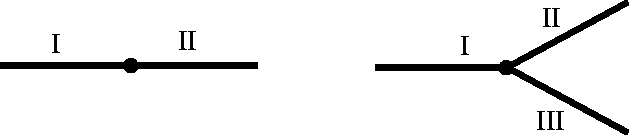
\includegraphics[width=0.6\linewidth]{bc_2.pdf}
    \caption{Локальная нумерация эелементов при рассмотрении сочленения}
    \label{fig:bc_2}
\end{figure}

C учётом выбранного направления движения $w_1$ слева направо
вычислим противопотоковые значения переменных Римана как
\begin{equation*}
\bar w_1 = u_I + 4 (c_I - c_0), \quad \bar w_2 = u_{II} - 4 (c_{II} - c_0), \quad \bar w_3 = u_{III} - 4 (c_{III} - c_0).
\end{equation*}
Значения $u,c_{I,II,III}$ - есть значение функций в точке сочленения, взятое
со стороны соответствующего элемента. Эти значения берутся с известного итерационного слоя.

При рассмотрения линейного сочленения (правый из рисунков \ref{fig:bc_2})
далее пользуясь определением \cref{eq:w12_def}
запишем уравнения
\begin{equation}
\label{eq:sys2}
\begin{aligned}
&\bar w_1 = \bar u_1 + 4 (\bar c_1 - c_0), \\
&\bar w_2 = \bar u_2 - 4 (\bar c_2 - c_0)
\end{aligned}
\end{equation}
В случае, если физические свойства ($\beta$ и $A$) не терпят разрыв в точке сочленения,
то $\bar u_1 = \bar u_2$, $\bar c_1 = \bar c_2$ и эта система
может быть разрешена с помощью выражений
\cref{eq:ua_from_w}. Иначе её следует дополнить двумя уравнениями сохранения: расхода и полного давления
\begin{equation}
\label{eq:sys1}
\begin{aligned}
&q(\bar u_1, \bar a_1) = q(\bar u_2, \bar a_2), \\
&P(\bar u_1, \bar a_1) = P(\bar u_2, \bar a_2)
\end{aligned}
\end{equation}
Нелинейная система \cref{eq:sys1,eq:sys2} может быть решена итерационным решателем (например, методом Ньютона).

В случае разветвления сосудов (правая схема на рис.~\ref{fig:bc_2}), аналогичная система уравнений,
дополненная условиями разрешимости на основе \cref{eq:q_conservation,eq:p_total_conservation} примет вид

\begin{equation}
\label{eq:sys3}
\begin{aligned}
&\bar w_1 = \bar u_1 + 4 (\bar c_1 - c_0), \\
&\bar w_2 = \bar u_2 - 4 (\bar c_2 - c_0), \\
&\bar w_3 = \bar u_3 - 4 (\bar c_3 - c_0), \\
&q(\bar u_1, \bar a_1) = q(\bar u_2, \bar a_2) + q(\bar u_3, \bar a_3), \\
&P(\bar u_1, \bar a_1) = P(\bar u_2, \bar a_2), \\
&P(\bar u_1, \bar a_1) = P(\bar u_3, \bar a_3).
\end{aligned}
\end{equation}
